\documentclass{zhslides}

\usepackage{logic}


\title{Day 3: 模糊性与多值逻辑}
\subtitle{}
\date{\today}
\date{2026年7月22日}
\author{于佳铭}
\institute{唯理书院2026\\「精确的逻辑与模糊的意义」} % or \textbf

\begin{document}

\maketitle

%\begin{frame}{目录}
%  \tableofcontents
%\end{frame}

% 可以用 \alert{} 来高亮


\begin{frame}{永真式}

  \bit
    \item \term{永真式/重言式}{tautology}：真值永远为真的语句
    \item \term{永假式/矛盾式}{contradiction}：真值永远为假的语句
  \eit

\end{frame}


\begin{frame}{经典逻辑的基本预设}

  \begin{law*}{二值原则, Bivalence}
    每个命题 $P$ 都有且只有一个真值。
  \end{law*}
  \pause
%  因此，根据 XXX，每个语句 $\phi$ 都有且只有一个真值。

  \begin{law*}{排中律, LEM}
    对于任意语句 $\phi$，$\phi \lor \neg \phi$ 是永真式。
  \end{law*}
  \pause

  \begin{law*}{矛盾律, LNC}
    对于任意语句 $\phi$，$\neg(\phi \land \neg \phi)$ 是永真式。
  \end{law*}
  
%  \begin{proposition*}{排中律, LEM}
%    对于任意语句 $p$，$p \lor \neg p$ 是永真式。
%  \end{proposition*}

\end{frame}


\begin{frame}[t]{二值原则的局限性}
  
  \vspace{2em}
  \begin{brainstorm*}{}
    是否真、假这两个二元的真值无法涵盖我们对于真值的认知？
  \end{brainstorm*}
  \vspace{1em}
  
  \pause
  \bit
    \item 模糊性：“张三是富有的”
    \item 逻辑悖论：“这句话是假的”
    \item 关于未来的不确定性：“明天将会下雨”
    \item 预设失败：“张三戒烟了”
    \item 虚构指称：“福尔摩斯的左腿上有一颗痣”
  \eit

\end{frame}




\section{谷堆悖论}

\begin{frame}{谷堆悖论}
  
  \begin{center}
    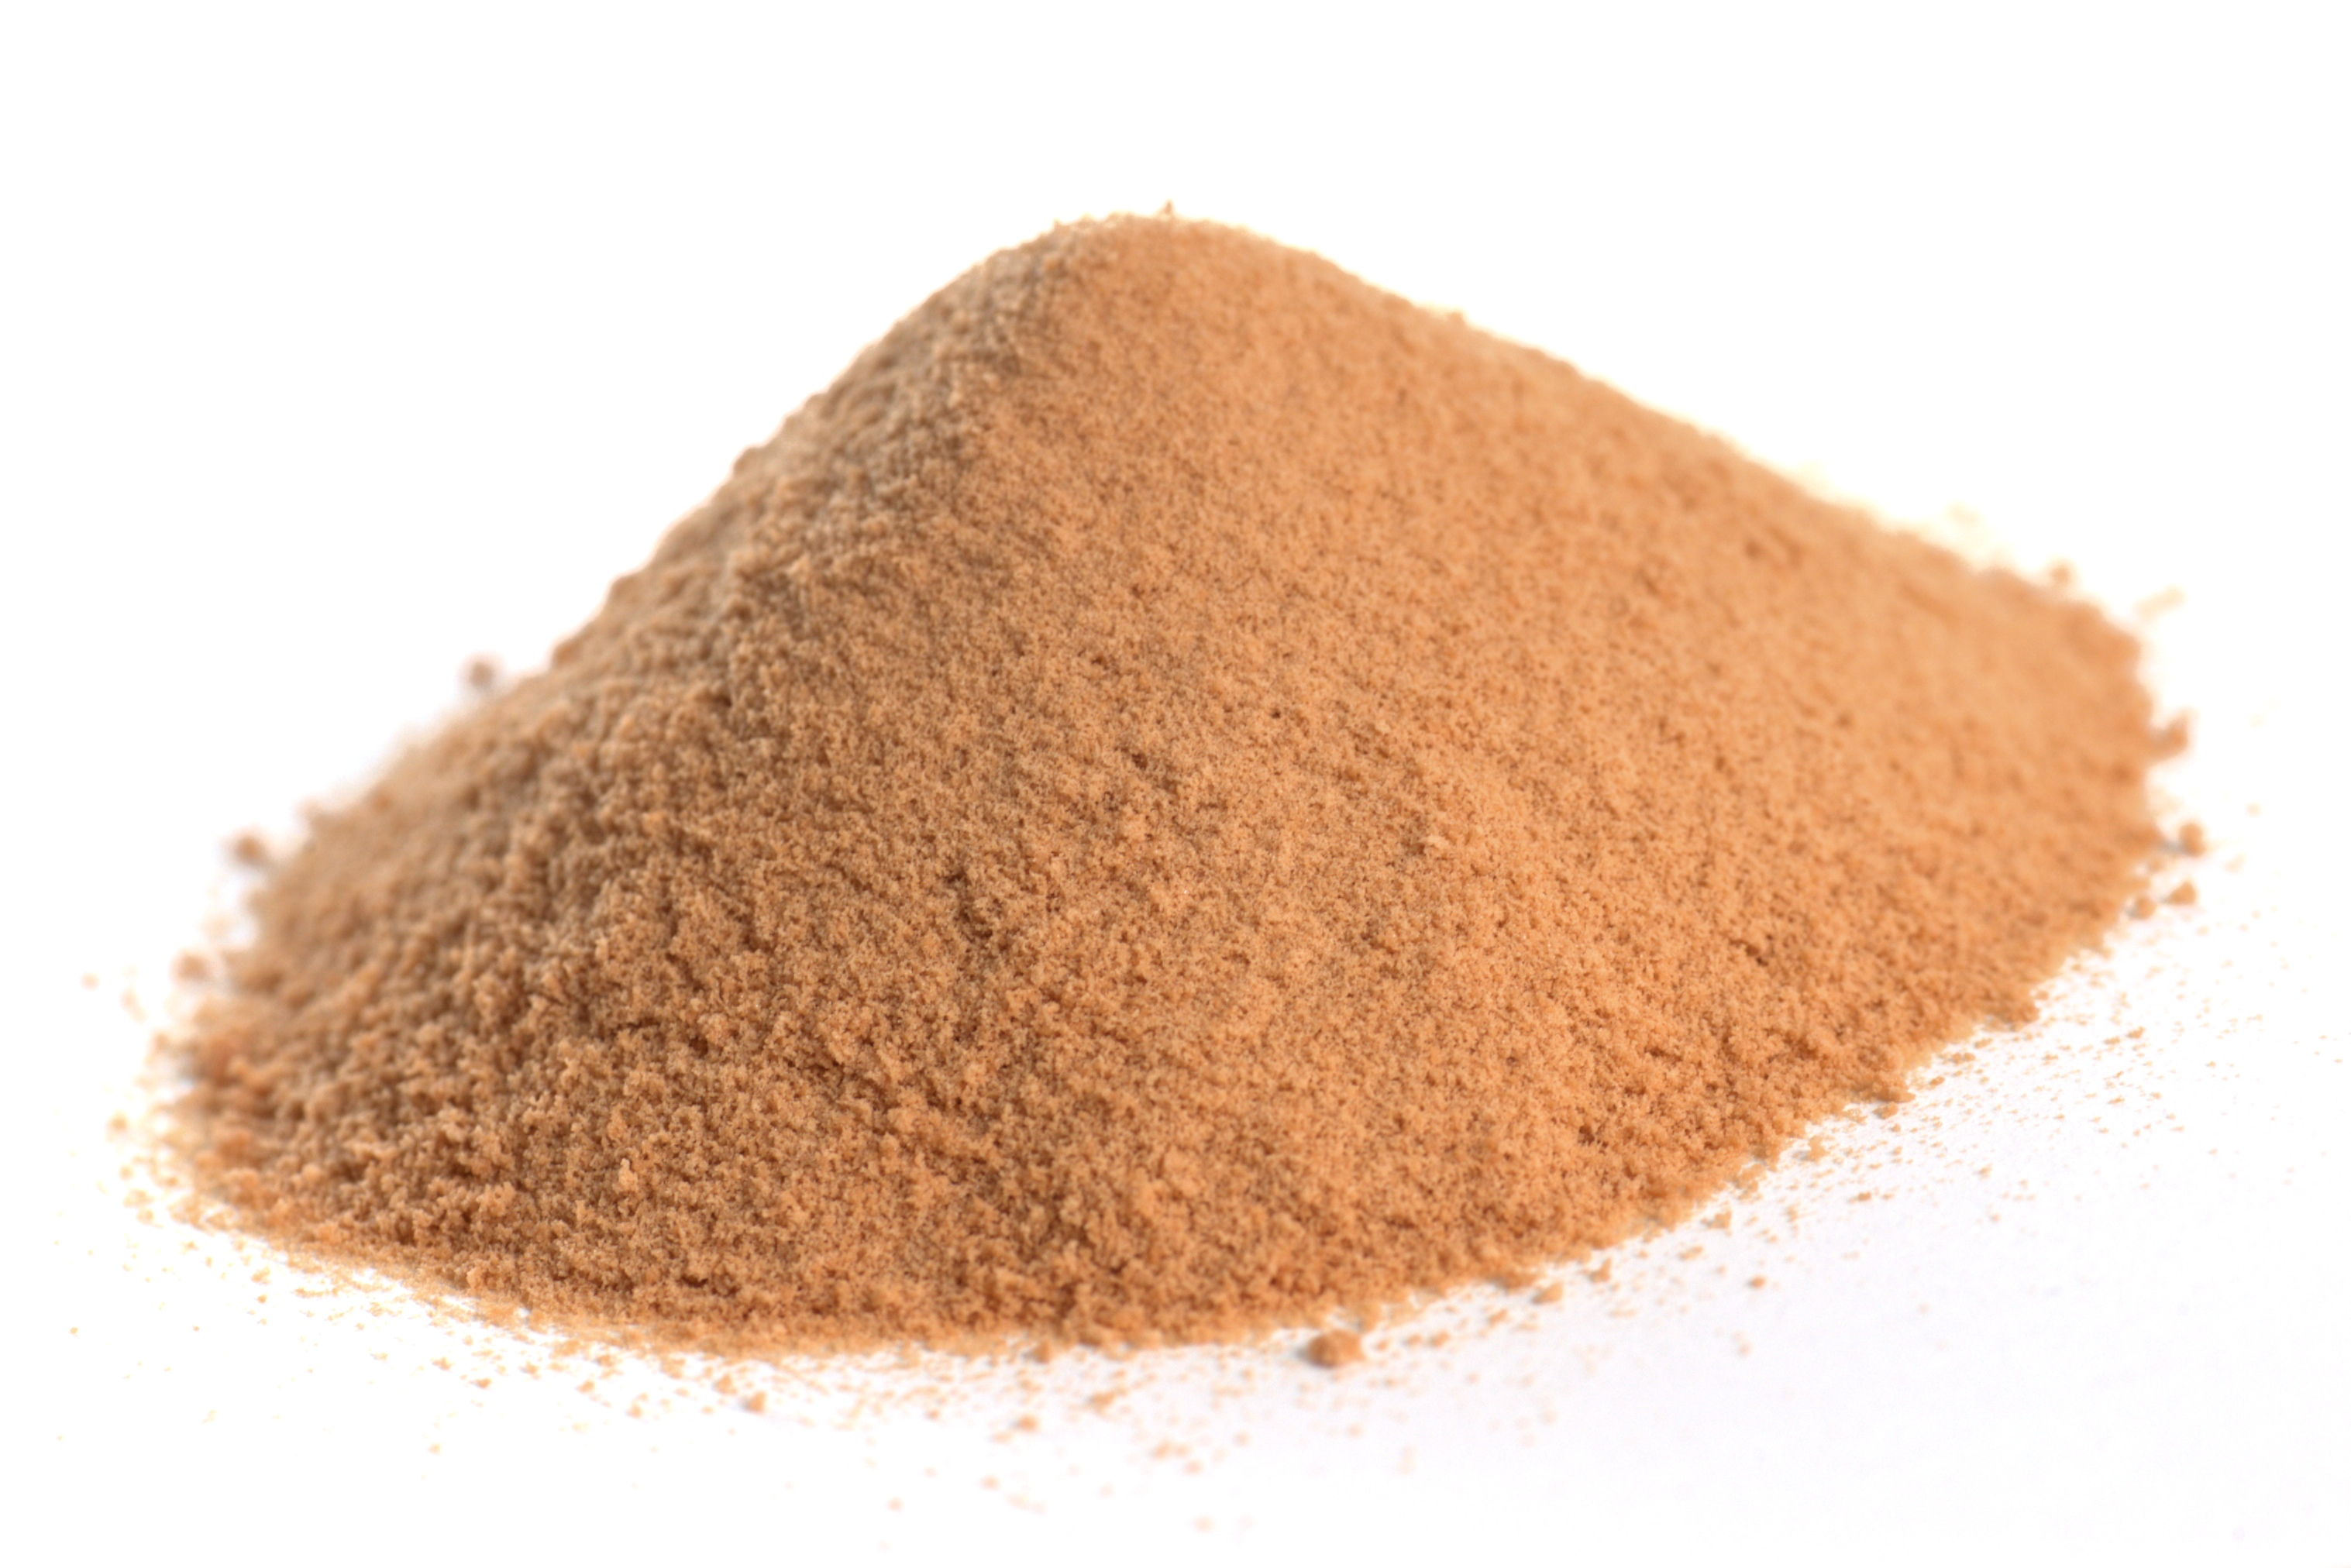
\includegraphics[width=0.5\textwidth]{images/heap.jpg}
  \end{center}
  
\end{frame}


\begin{frame}{谷堆悖论}
  
  论证：
  \begin{enumerate}
    \item 1粒谷子不构成谷堆
    \item 如果$n$粒谷子不构成谷堆，那么$n + 1$粒谷子也不构成谷堆
  \end{enumerate}
  因此：
  \begin{enumerate}
    \setcounter{enumi}{2}
    \item \num{1000000}粒谷子也不构成谷堆
    \pause
    \item 任意数量的谷子都不构成谷堆
  \end{enumerate}
  
\end{frame}


\begin{frame}{谷堆悖论}
  
  我们为什么要在意这个奇怪的悖论？
  \bit
    \item 这样的模糊谓词无处不在：“高”、“秃”、“年轻”
    \item 他们表面上看也一样是可以判断真假的陈述句
    \item 逻辑体系和自然语言的直觉之间的张力
%    \bi
%      \item 当我们否认“A是高的” $\neq$ “A具有不高的属性”
%    \ei
  \eit
  
\end{frame}


\begin{frame}{谷堆悖论}
  
  如何回应谷堆悖论？
  \begin{enumerate}
    \item 1粒谷子不构成谷堆
    \item 如果$n$粒谷子不构成谷堆，那么$n + 1$粒谷子也不构成谷堆
  \end{enumerate}
  
  \pause
  \vspace{2em}
  \begin{brainstorm*}{}
    我们应该否认前提1、否认前提2、还是修改逻辑系统本身？
  \end{brainstorm*}
  
\end{frame}


%\begin{frame}{两栏布局}
%  \begin{columns}[T]
%    \begin{column}{0.48\textwidth}
%      \textbf{左栏内容}
%      \begin{itemize}
%        \item 第一点
%        \item 第二点
%        \item 第三点
%      \end{itemize}
%    \end{column}
%    \begin{column}{0.48\textwidth}
%      \textbf{右栏内容}
%      \begin{itemize}
%        \item First item
%        \item Second item
%        \item Third item
%      \end{itemize}
%    \end{column}
%  \end{columns}
%\end{frame}




\section{多值逻辑}

\begin{frame}{武卡谢维奇逻辑}
  
  \bi
    \item 武卡谢维奇（{\L}ukasiewicz）在1920年提出第一个三值逻辑\footnote<4->[frame]{完整的武卡谢维奇逻辑允许连续的真值，在那样的定义下，$\phi \implies \psi$的真值被自然地定义为$\min(1, 1 - \phi + \psi)$}
    \item 引入了“不确定”的真值：$\hash$
    \item 真值集合：$\settfh$或者$\set{1, 0, \hash}$
  \ei
  \pause
  
  \begingroup
  \setlength{\tabcolsep}{4pt}
  \begin{table}[h]
  \centering
  \begin{tabular}{c|c}
    $\neg$ & \\\hline
    1 & 0 \\
    0 & 1 \\
    \hash & \hash
  \end{tabular}
  \quad
  \begin{tabular}{c|ccc}
    $\land$ & 1 & 0 & \hash \\\hline
    1 & 1 & 0 & \hash \\
    0 & 0 & 0 & 0 \\
    \hash & \hash & 0 & \hash
  \end{tabular}
  \quad
  \begin{tabular}{c|ccc}
    $\lor$ & 1 & 0 & \hash \\\hline
    1 & 1 & 1 & 1 \\
    0 & 1 & 0 & \hash \\
    \hash & 1 & \hash & \hash
  \end{tabular}
  \quad
  \begin{tabular}{c|ccc}
    $\implies$ & 1 & 0 & \hash \\\hline
    1 & 1 & 0 & \hash \\
    0 & 1 & 1 & 1 \\
    \hash & 1 & \hash & \only<2>{1}\only<3->{\hl{\,1\,}}
  \end{tabular}
  \end{table}
  \endgroup
  
\end{frame}


%\begin{frame}{武卡谢维奇逻辑：逻辑有效性}
%
%  \bit
%    \item 当我们引入了新的真值，我们也要同时考虑逻辑有效性和逻辑结果的定义
%    \item 对于一个真值集合$\mathcal{V}$，我们可以选取其某一子集$\mathcal{V}^*$作为\term{指定真值}{designated truth values}
%    \item 则，逻辑有效性即可被定义为“永远指定真”；逻辑结果可以被定义为“保指定真性”
%  \eit
%
%\end{frame}


\begin{frame}{克莱尼真值表}

  \bi
    \item 克莱尼（Kleene）修改了武卡谢维奇逻辑中$(\hash \implies \hash)$的真值
  \ei
  
  \begingroup
  \setlength{\tabcolsep}{4pt}
  \begin{table}
  \centering
  \begin{tabular}{c|c}
    $\neg$ & \\\hline
    1 & 0 \\
    0 & 1 \\
    \hash & \hash
  \end{tabular}
  \quad
  \begin{tabular}{c|ccc}
    $\land$ & 1 & 0 & \hash \\\hline
    1 & 1 & 0 & \hash \\
    0 & 0 & 0 & 0 \\
    \hash & \hash & 0 & \hash
  \end{tabular}
  \quad
  \begin{tabular}{c|ccc}
    $\lor$ & 1 & 0 & \hash \\\hline
    1 & 1 & 1 & 1 \\
    0 & 1 & 0 & \hash \\
    \hash & 1 & \hash & \hash
  \end{tabular}
  \quad
  \begin{tabular}{c|ccc}
    $\implies$ & 1 & 0 & \hash \\\hline
    1 & 1 & 0 & \hash \\
    0 & 1 & 1 & 1 \\
    \hash & 1 & \hash & \hl{\hash}
  \end{tabular}
  \end{table}
  \endgroup
  
  \pause  
  \bi
    \item 原则：如果一个式子里的经典真值有足够信息来确定式子的经典真值，则该真值就是式子的真值，否则式子的真值是$\hash$
  \ei

\end{frame}


\begin{frame}{三值逻辑：批判}

  \begin{brainstorm*}{}
    请举例一个在武卡谢维奇逻辑里永真但在克莱尼逻辑里不永真的式子。
  \end{brainstorm*}
  
  \begin{brainstorm*}{}
    请给出克莱尼逻辑里任何一个永真式，或者证明不存在任何永真式。
  \end{brainstorm*}
  
  \begin{brainstorm*}{}
    三值逻辑可以帮我们解释/解决谷堆悖论吗？
  \end{brainstorm*}
  \vspace{-0.5em}
  \pause
  $\quad\rightarrow$ 高阶模糊性
  
\end{frame}



\section{超赋值理论}

\begin{frame}{精细化}
  
  \bit
    \item 模糊谓词的模糊性来源于不同但都合理的边界划分方式
    \item 每一种划分边界的方式都是一种\term{精细化}{precisification}
  \eit
  
\end{frame}


\begin{frame}{超赋值理论}
  
  \begin{definition*}{超真性}
    一个语句$\phi$是\term{超真}{supertrue}的，当且仅当$\phi$在\em{所有}容许的精细化下都为真。
  \end{definition*}
  \pause
  
  \begin{definition*}{超假性}
    一个语句$\phi$是\term{超假}{superfalse}的，当且仅当$\phi$在\em{所有}容许的精细化下都为假。
  \end{definition*}
  \pause
  
  若$\phi$在有些精细化下为真、有些为假，那么$\phi$既非超真也非超假。
  \pause
  但这种既非又非的状态不等同于$\hash$，不作为一种真值参与计算。
  
\end{frame}


\begin{frame}{超赋值理论 vs 三值逻辑}
  
  \begin{brainstorm*}{}
    超赋值理论可以规避高阶模糊性的问题吗？
  \end{brainstorm*}
  
\end{frame}







\end{document}